\section{Choix et Conception}
    
    \subsection{Choix du dispositif}
    
        Pour notre projet, nous avons choisit Raspbery pi, pour la facilité qu'il nous offre, car le raspberry pi est un véritable ordinateur sur lequel on peut installer un système d'exploitation, écrire des programmes dans plusieurs langages et même installer un serveur web. On peut aussi brancher des périphériques et un câble réseau.

    \subsection{Choix des capteurs}
    
        Nous avons choisi nos capteurs en se basant sur plusieurs critères : compatibilté avec le Raspberry, les besoins de notre projet, prix, disponibilité, etc.
        
        \begin{center}
        \begin{tabular}{ c c c }
         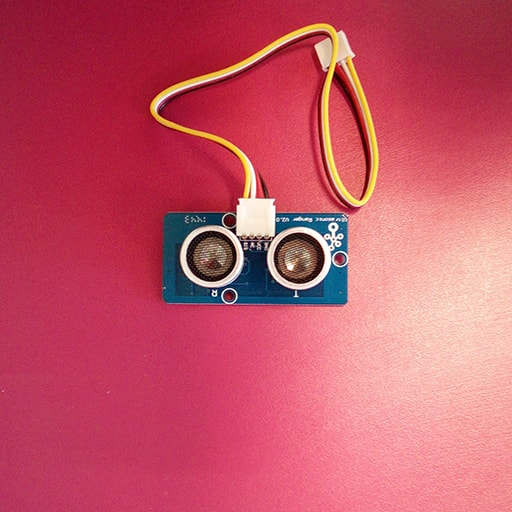
\includegraphics[height=2.5cm]{ultrasonic.jpg} & 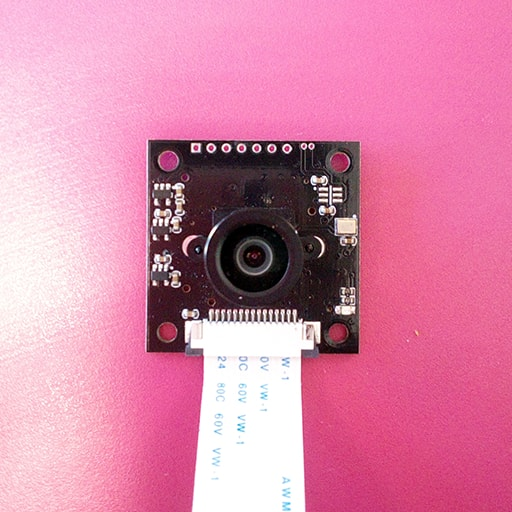
\includegraphics[height=2.5cm]{camera.jpg} & 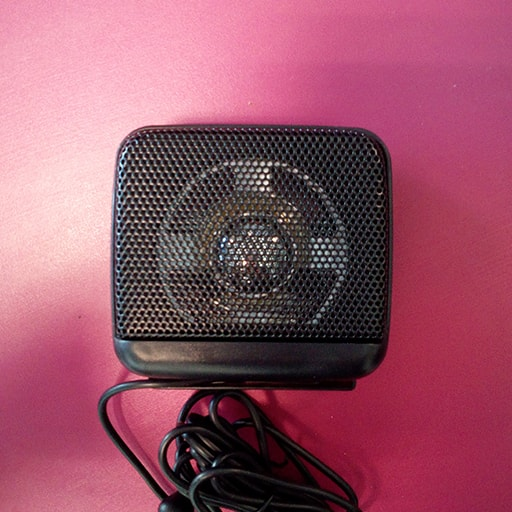
\includegraphics[height=2.5cm]{speakers.jpg} \\ 
         Capteur Ultrason Groove & Camera nocturne PI-NoIR & Haut Parleurs \\   
        \end{tabular}
        \end{center}
        
        \begin{itemize}
            \item \textbf{Capteur Ultrason Groove : }permet de mesurer la distance sans contact à l'aide de transducteurs à ultrasons. Ce capteur a une portée de 4 mètres ce qui est idéal pour notre projet.
            \item \textbf{PI-NoIR : }Une caméra sans filtre infrarouge, idéal pour la vision nocturne avec un grand angle de couverture de 105°, une connexion CSI, et un prix très raisonnable (30 euros).
            \item \textbf{Hauts parleurs : } simples, faciles à monter et à un prix raisonnable. Alimenté avec le cable jack et (pas besoin de batteries). Le seul inconvénient de ces hauts parleurs est que leurs volume est bas.
        \end{itemize}
        
    \subsection{Architecture}
    \includegraphics[width=15cm]{architecture.png}